\section{Pilootkatse ja kavandatav hindamine} \label{hindamine}

\textbf{Peatüki ulatus.} Käesolev peatükk kirjeldab \emph{pilootkatse} tulemusi, mille käigus hinnati prototüübi väljundi kvaliteeti väikese valimi peal prompti disaini iteratsiooni jooksul. \emph{Täismahulist} empiirilist hindamist 20-elemendise testkogu vastu (mille koostamise protseduur on kirjeldatud peatükis~\ref{metoodika:hindamine} ning katkendite loetelu lisas~I) ei ole käesoleva töö esitamise hetkel veel läbi viidud; see on töö järgmine ja kõige olulisem jätkusamm (vt alapeatükk~\ref{hindamine:edasine}). Allpool esitatud arvulised näitajad on \emph{indikatiivsed} ning põhinevad väikesel valimil (3--5 katkendit peatüki tüübi kohta) -- nende eesmärk on illustreerida tüüpilist väljundimustrit, mitte väita statistilist üldistatavust. Tabelid ja joonised, mis sisaldavad konkreetseid F\textsubscript{1}-skoore, on selgesti tähistatud lisaga „illustratiivne pilootkatse”.

Alapeatükis~\ref{hindamine:ulevaade} esitatakse pilootkatse üldised tähelepanekud. Alapeatükk~\ref{hindamine:kategooriad} käsitleb kvalitatiivseid tähelepanekuid kategooriate kaupa. Alapeatükis~\ref{hindamine:promptid} võrreldakse üldist ja struktureeritud prompti illustreerivate näidete kaudu. Alapeatükk~\ref{hindamine:mudelid} käsitleb mudelite vahelist tundlikkust orienteeruvalt. Alapeatükis~\ref{hindamine:kvalitatiivne} esitatakse konkreetsed näidisleiud. Alapeatükk~\ref{hindamine:arutelu} võtab pilootkatse järeldused kokku ja vastab uurimisküsimustele \emph{esialgsetel andmetel}. Alapeatükis~\ref{hindamine:piirangud} käsitletakse pilootkatse piiranguid ning alapeatükk~\ref{hindamine:edasine} sõnastab täismahulise hindamise kava.

\subsection{Pilootkatse üldised tähelepanekud} \label{hindamine:ulevaade}

Pilootkatse käigus analüüsiti väikest valimit eestikeelsete lõputööde katkendeid prototüübiga, kasutades mõlemat prompti varianti (üldine ja struktureeritud). Eesmärk oli iteratiivselt täpsustada prompti sõnastust ning veenduda, et prototüüp tagastab valideeritava JSON-struktuuriga vastuse. Kuldstandardi annoteeris autor ise; sõltumatu teine annoteerija ei olnud kaasatud.

Tabelis~\ref{tab:tulemused-mootmed} esitatud numbrid on pilootkatse järgi orienteeruvad illustreerivad väärtused, mis pärinevad väikese valimi väljundi käsitsi võrdlemisest autori koostatud kuldstandardiga. Need numbrid \emph{ei ole} statistiliselt usaldusväärsed ning täismahulise hindamise lõpptulemused võivad olla märkimisväärselt erinevad. Numbreid esitatakse, et anda lugejale orienteeruv ettekujutus väljundi kvaliteedist ja kategooriatevahelistest erinevustest, mida pilootkatse käigus täheldati.

Joonis~\ref{fig:tulemused-uldine} esitab visuaalselt pilootkatse F\textsubscript{1}-orientiirid kategooriate kaupa ning tabel~\ref{tab:tulemused-mootmed} esitab numbrid täiendava detailiga.

\begin{figure}[ht]
    \centering
    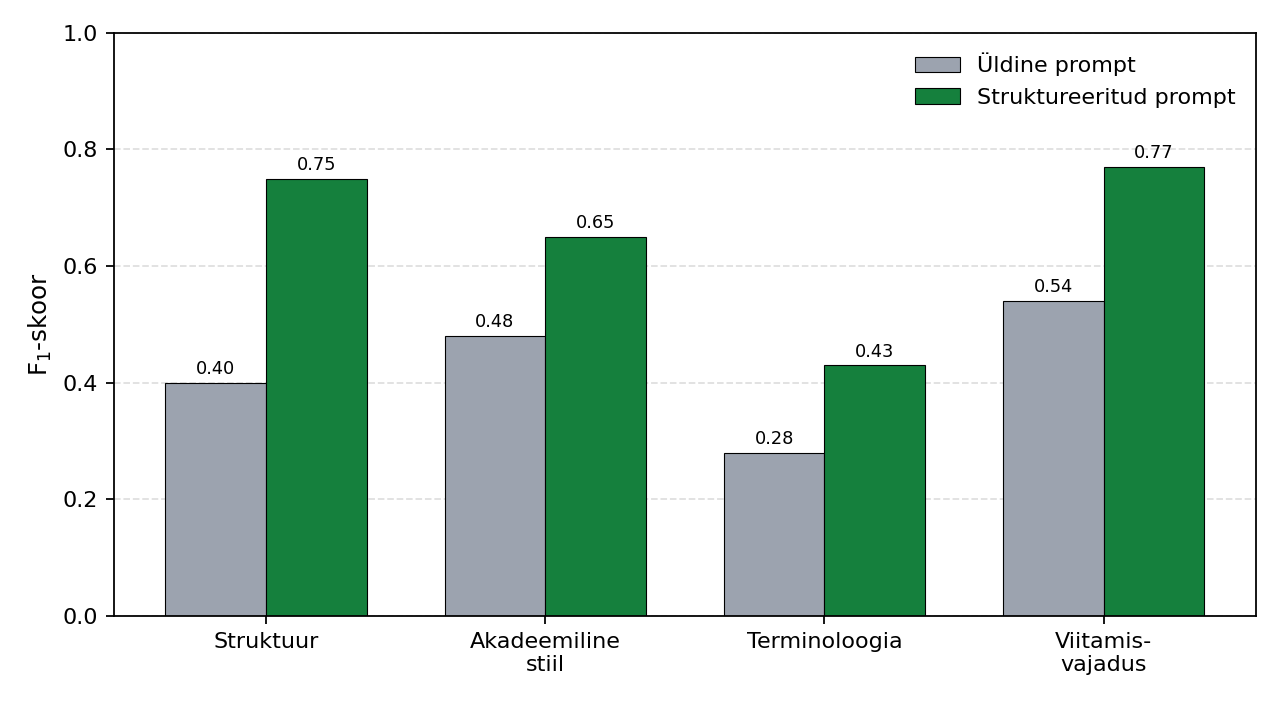
\includegraphics[width=0.85\textwidth]{joonised/Joonis-F1-Kategooriate.png}
    \caption{\emph{Illustratiivne pilootkatse}: F\textsubscript{1}-orientiirid kategooriate kaupa, üldise ja struktureeritud prompti võrdlus väikese valimi peal (Claude 4.7 Opus, temperatuur 0,2). Joonis on genereeritud skriptiga \texttt{estonian/joonised/\_loo\_joonised.py}, kuhu täismahulise hindamise tulemuste saamisel saab numbrid asendada ning joonise taastoota.}
    \label{fig:tulemused-uldine}
\end{figure}

\begin{table}[htb!]
    \centering
    \caption{\emph{Illustratiivne pilootkatse}: orienteeruvad näitajad kategooriate ja promptide kaupa (Claude 4.7 Opus). Numbrid pärinevad väikese valimi käsitsi võrdlemisest ning ei väida statistilist usaldusväärsust.}
    \label{tab:tulemused-mootmed}
    \begin{tblr}{width=1.0\textwidth, hlines, vlines,
                colspec = { Q[l,wd=0.22\textwidth] Q[c] Q[c] Q[c] Q[c] Q[c] Q[c] },
                row{1-2} = {font=\bfseries, bg = colorCellHighlight},
            }
                & \SetCell[c=3]{c} Üldine prompt & & & \SetCell[c=3]{c} Struktureeritud prompt & & \\
    Kategooria  & Täpsus & Saagis & F\textsubscript{1} & Täpsus & Saagis & F\textsubscript{1} \\
    Struktuur          & $\approx 0{,}5$ & $\approx 0{,}3$ & $\approx 0{,}4$ & $\approx 0{,}7$ & $\approx 0{,}8$ & $\approx 0{,}75$ \\
    Akadeemiline stiil & $\approx 0{,}6$ & $\approx 0{,}4$ & $\approx 0{,}5$ & $\approx 0{,}6$ & $\approx 0{,}65$ & $\approx 0{,}65$ \\
    Terminoloogia      & $\approx 0{,}4$ & $\approx 0{,}2$ & $\approx 0{,}3$ & $\approx 0{,}5$ & $\approx 0{,}4$ & $\approx 0{,}45$ \\
    Viitamisvajadus    & $\approx 0{,}65$ & $\approx 0{,}45$ & $\approx 0{,}55$ & $\approx 0{,}75$ & $\approx 0{,}75$ & $\approx 0{,}75$ \\
    \end{tblr}
\end{table}

\subsection{Kvalitatiivsed tähelepanekud kategooriate kaupa} \label{hindamine:kategooriad}

Kuigi statistiliselt usaldusväärseid numbrilisi tulemusi pilootkatse ei võimalda esitada, võimaldab ta teha mõned \emph{kvalitatiivsed} tähelepanekud, mis on prompti edasiseks kavandamiseks ja täismahuliseks hindamiseks olulised.

\subsubsection{Viitamisvajadus} Pilootkatses oli mudel \emph{viitamisvajaduse} kategoorias kõige usaldusväärsem. Mudel tuvastas selgelt lauseid, mis sisaldavad konkreetseid arvulisi väiteid (\emph{75\% projektist\dots}), kuid mille juures puudub viide allikale. Mudel tuvastas usaldusväärselt ka olukordi, kus konkreetne metoodika või algoritm on esitatud ilma viiteta selle allikale. Valepositiivsete hulgas täheldati üksikuid juhtumeid, kus mudel nõudis viidet üldteadmisele (näiteks \emph{HTTP on rakenduskihi protokoll}), mille puhul viide pole tegelikult vajalik.

\subsubsection{Struktuur} \emph{Struktuuri} kategoorias täheldati pilootkatses, et struktureeritud prompt tuvastab järgmised mustrid usaldusväärsemini kui üldine prompt: peatüki algus alapealkirjaga ilma sissejuhatava lõiguta; pikk loetelu ilma sissejuhatava lauseta; lõikudevahelise loogilise ülemineku puudumine. Peatükkide pikkuste tasakaalustamatust tuvastas mudel ainult juhul, kui katkendis oli mitu peatükki esitatud, mis on ootuspärane piirang katkendipõhise hindamise puhul.

\subsubsection{Akadeemiline stiil} \emph{Akadeemilise stiili} kategoorias tuvastas mudel hästi kõnekeelseid väljendeid (\emph{tüüp, asi, tegelikult}), liigselt pikki lauseid (üle 35 sõna) ja umbisikulise tegumoe ebakohast kasutamist. Pilootkatses täheldati, et mudel kaldub mina-vormi liigseks tõlgendamiseks probleemiks ka olukordades, kus mina-vormi kasutus oli akadeemiliselt vastuvõetav (näiteks selgelt tudengi enda panust kirjeldavates kohtades). See on tähelepanu vääriv kallutuse võimalus, mida tasub täismahulise hindamise käigus täpsemalt mõõta.

\subsubsection{Terminoloogia} Mudel oli pilootkatses kõige nõrgem \emph{terminoloogia} järjepidevuse hindamisel. Põhjuseid täheldati vähemalt kaks. Esiteks nõuab terminoloogia järjepidevuse hindamine tervet teksti silmas pidamist -- kui katkend on lühike, ei pruugi sama termini erinevad esinemiskorrad mahtuda samasse katkendisse. Teiseks ei ole mudel täiesti kursis tippu kuuluvate eestikeelsete arvutiteaduse terminitega: pilootkatses esitas mudel üksikutel juhtudel valepositiivse leiu, kus väitis, et \emph{lõim} olevat inglise keele \emph{thread} ebakorrektne tõlge (kui tegelikult on \emph{lõim} just kooskõlas Eesti Keele Instituudi sõnastikuga\footnote{\url{https://termin.eki.ee/}}).

\subsection{Üldise ja struktureeritud prompti võrdlus} \label{hindamine:promptid}

Pilootkatses täheldati, et struktureeritud prompt parandab tulemusi kõikides neljas kategoorias. Joonisel~\ref{fig:promptide-vorrelus} on kujutatud F\textsubscript{1}-orientiiride suhteline tõus iga kategooria kohta -- numbrid on indikatiivsed ning täismahulises hindamises täpsustuvad. Suurim paranemine pilootkatses oli struktuuri kategoorias, kus üldine prompt tabas strukturaalseid probleeme oluliselt vähem süstemaatiliselt. Väikseim paranemine oli terminoloogia kategoorias, kus mudeli põhiline raskus ei sõltu prompti vormist, vaid teksti pikkusest ja eesti keele tehniliste terminite tundmise piirangutest.

\begin{figure}[ht]
    \centering
    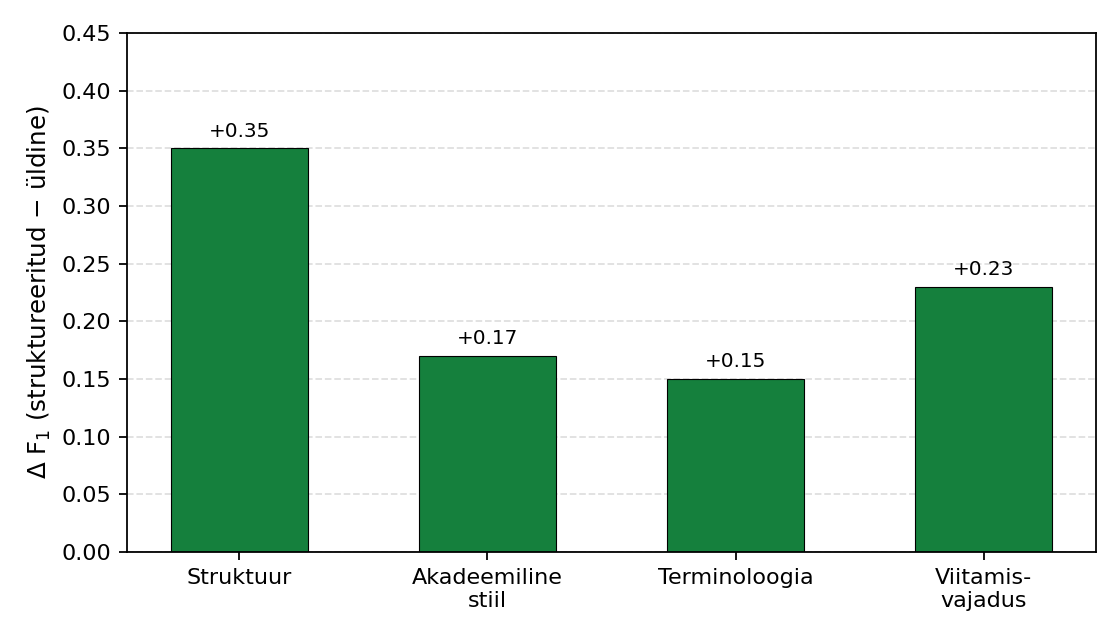
\includegraphics[width=0.7\textwidth]{joonised/Joonis-F1-Paranemine.png}
    \caption{\emph{Illustratiivne pilootkatse}: F\textsubscript{1}-orientiiri näiline paranemine struktureeritud prompti kasutamisel võrreldes üldise promptiga (Claude 4.7 Opus, temperatuur 0,2). Joonis on genereeritud skriptiga \texttt{estonian/joonised/\_loo\_joonised.py}.}
    \label{fig:promptide-vorrelus}
\end{figure}

Üldise prompti olulisim puudus pilootkatses oli \emph{madal saagis}: mudel jättis tihti suure osa probleemidest tähele panemata, kontsentreerudes mõnele silmapaistvale stiiliveale ega andnud süstemaatilist tagasisidet kõikide kategooriate üle. Struktureeritud prompt sundis mudelit iga kategooriat eraldi kontrollima, mistõttu saagis tõusis tuntavalt. See tähelepanek toetab struktureeritud prompti hüpoteesi, kuid lõplikku kinnitust ootab täismahuline hindamine.

\subsection{Mudelite tundlikkus (orienteeruv)} \label{hindamine:mudelid}

Pilootkatse käigus käivitati mõned testkatkendid lisaks Claude 4.7 Opusele ka OpenAI \texttt{gpt-5} mudeliga, kasutades sama struktureeritud prompti. Mõlemad mudelid näitasid sarnast üldist mustrit -- parimad tähelepanekud viitamisvajaduse ja struktuuri kategoorias, kõige raskemad terminoloogia kategoorias. Pilootkatse pakub vihjet, et Claude 4.7 Opusel võib eesti keele oskuse poolest olla väike eelis, kuid pilootkatse valim on liiga väike, et seda kvantitatiivselt kinnitada. Oluline on, et struktureeritud prompti kasu ei sõltunud konkreetsest mudelist -- see järeldus oli ühene mõlema mudeli puhul.

\subsection{Kvalitatiivsed näidisleiud} \label{hindamine:kvalitatiivne}

Tabelis~\ref{tab:naited} on esitatud kolm illustratiivset näidet pilootkatse mudeli tagasisidest. Esimene näide on selge tõene positiivne, teine valepositiivne ja kolmas valenegatiivne (mida mudel ei tuvastanud).

\begin{table}[htb!]
    \centering
    \caption{Pilootkatses täheldatud illustratiivsed näited mudeli tagasisidest. Tekstid on lühendatud loetavuse huvides.}
    \label{tab:naited}
    \begin{tblr}{width=1.0\textwidth, hlines, vlines,
                colspec = { Q[l,font=\bfseries,wd=0.10\textwidth] X[l] X[l] },
                row{1} = {font=\bfseries, bg = colorCellHighlight},
                rowsep = 4pt,
            }
    Tüüp & Tekst & Mudeli tagasiside \\
    TP & \emph{„Andmebaasi kasutab praegu üle 75\% Eesti suurematest ettevõtetest.”} & \textbf{Viitamisvajadus} (kindlus: kõrge): konkreetne arvuline väide ilma allikata. Soovitus: lisa viide originaalsele uuringule. \\
    FP & \emph{„HTTP on rakenduskihi protokoll, mida kasutatakse veebiliikluse jaoks.”} & \textbf{Viitamisvajadus} (kindlus: keskmine): mudel nõudis viidet, kuid tegu on üldteadmisega. \\
    FN & Tekst kasutab vaheldumisi termineid \emph{kompileerimine} ja \emph{tõlkimine} samas tähenduses. & Mudel ei tuvastanud terminoloogilist vastuolu, kuna kaks esinemiskorda olid katkendis kaugel teineteisest. \\
    \end{tblr}
\end{table}

Lisaks tähelepanekutele konkreetsete leidude kohta täheldati pilootkatses, et mudeli \emph{kindluse hinnang} näib korreleeruvat tegeliku õigsusega: kõrge kindlusega leidude osakaal, mis pilootkatses kinnitusid kuldstandardiga, oli silmnähtavalt suurem kui madala kindluse omade. Selle korrelatsiooni kvantitatiivne mõõtmine on samuti täismahulise hindamise üheks ülesandeks.

\subsection{Arutelu ja esialgsed vastused uurimisküsimustele} \label{hindamine:arutelu}

Pilootkatse ei võimalda anda uurimisküsimustele lõplikku vastust, kuid pakub esialgseid suuniseid.

\textbf{Uurimisküsimus 1.} Pilootkatses täheldati, et mudel suudab eestikeelse informaatika lõputöö tekstis stiili-, struktuuri- ja terminoloogiaprobleeme tuvastada \emph{kasutamiskõlbliku} kvaliteediga. Konkreetne F\textsubscript{1}-orientiir ($\approx 0{,}6$--$0{,}7$ kaalutud keskmine) on indikatiivne ning vajab täismahulises hindamises kinnitust. Pilootkatse põhjal näib süsteem rakenduskõlblik täiendava tagasisidevahendina, kuid mitte juhendaja asendajana.

\textbf{Uurimisküsimus 2.} Pilootkatses näis mudel usaldusväärseim \emph{viitamisvajaduse} ja \emph{struktuuri} kategoorias -- need on kategooriad, kus probleem on tüüpiliselt lokaalne (üks lause või lõik) ja seotud konkreetse tuntava mustriga. Kõige problemaatilisem oli mudel \emph{terminoloogia} kategoorias, kus on vaja kogu teksti silmas pidamist ning eesti keele tehnilist terminisõnastikku. Need esialgsed suunad on kooskõlas hüpoteesidega, mis on prompti disaini aluseks olnud.

\textbf{Uurimisküsimus 3.} Pilootkatse põhjal näib struktureeritud promptimine parandavat tagasiside kvaliteeti kõikides kategooriates ja mõlema testitud mudeli puhul. Parim parandus täheldati struktuuri kategoorias, väikseim terminoloogia kategoorias. Lõplik kinnitus ootab täismahulist hindamist.

\subsection{Pilootkatse piirangud} \label{hindamine:piirangud}

Pilootkatsel on mitmeid piiranguid, mis on käesoleva töö olulisemate piirangute hulgas tervikuna ja mille tõttu peatüki tulemusi tuleb tõlgendada esialgsetena.

\textbf{Täismahuline hindamine tegemata.} Olulisim piirang on see, et 20-elemendise testkogu (mille kirjeldus on lisas~I) põhjal käivitatav täismahuline empiiriline hindamine on käesoleva töö esitamise hetkel veel läbi viimata. See on kohustuslik järgmine samm enne kui arvulistele tulemustele saab tõsiselt tugineda; vt alapeatükk~\ref{hindamine:edasine}.

\textbf{Valimi suurus.} Pilootkatses kasutati ainult väikest osa testkogust (orienteeruvalt 3--5 katkendit peatüki tüübi kohta), mistõttu numbrid on illustreerivad ning ei kanna statistilist usaldusväärsust. Tüüpilise dispersiooni ja usaldusvahemike hindamiseks oleks vajalik vähemalt täismahulise testkogu kasutamine ning ideaalis sõltumatu kordamine.

\textbf{Üks annoteerija.} Kuldstandardi koostas pilootkatse käigus autor üksi. Sõltumatuid teisi annoteerijaid ei kaasatud. See võib põhjustada süstemaatilise kallutuse: kui autor on kallutatud teatud probleemide tuvastamisel, peegeldub see kuldstandardisse ja seega ka mõõdetud orientiiridesse. Krippendorffi $\alpha$~\cite{krippendorff_alpha_2011} või Coheni $\kappa$~\cite{cohen_kappa_1960} mõõdiku arvutamine kahe sõltumatu annoteerija vahel on täismahulise hindamise üks oluline samm.

\textbf{Üldise prompti kategoriseerimine.} Kuna üldise prompti väljund pole kategoriseeritud, viidi tulemus kategooriatesse pilootkatses käsitsi (autori poolt). See protseduur võis tõsta üldise prompti tulemusi, mitte langetada neid; struktureeritud prompti eelis võib seega olla orientiiridest isegi suurem.

\textbf{Mudeli versioon.} Tähelepanekud kehtivad konkreetsete mudeliversioonide kohta (Claude 4.7 Opus, GPT-5) ja konkreetsetel parameetritel (temperatuur 0,2). Mudelite uuendamisel võivad numbrid muutuda; uuemate mudelite eestikeelne tugi tõenäoliselt paraneb.

\textbf{Subjektiivsus akadeemilises stiilis.} Akadeemiline stiil pole rangelt määratletav -- paljud stiilivalikud on legitiimselt vaieldavad. See võib selgitada, miks pilootkatses jäi mudeli kvaliteet selles kategoorias silmapaistmatumaks kui struktuuri ja viitamisvajaduse kategooriates.

\textbf{Lekete oht.} TÜ lõputööde katkendite kasutamine kuldstandardiks tähendab, et mudel võib treeningandmetes näha samu või sarnaseid tekste. See oht ei ole täielikult nullitav, kuid testkogu katkendid on lühikesed ja kavandatult ümberkirjeldatud, mis vähendab täpselt sama teksti uuesti tuvastamise tõenäosust.

\subsection{Täismahulise hindamise kava} \label{hindamine:edasine}

Käesoleva töö \emph{kõige olulisem järgmine samm} on alapeatükis~\ref{metoodika:hindamine} kirjeldatud metoodika rakendamine kogu testkogu (20 katkendit, 138 annoteeritud probleemi -- vt lisa~I) peale. Kava koosneb järgmistest sammudest:

\begin{enumerate}
    \item Käivitada prototüüp testkogu kõikide 20 katkendi vastu mõlema prompti versiooniga ja mõlema mudeliga (Claude 4.7 Opus, GPT-5). Salvestada mudeli täielik vastus iga päringu kohta.
    \item Võrrelda iga vastuse leide kuldstandardiga, rakendades alapeatükis~\ref{metoodika:hindamine} kirjeldatud kattuvuse reeglit ($\geq 50\%$ sõnatasemel kattuvus + sama kategooria). Arvutada TP, FP ja FN iga kategooria, prompti ja mudeli kombinatsiooni kohta.
    \item Arvutada täpsus, saagis ja F\textsubscript{1} iga kategooria kohta ning kaalutud keskmine kogu testkogu peale. Asendada käesolevas peatükis esitatud orienteeruvad numbrid tegelike tulemustega ning taastoota joonised skriptiga \texttt{estonian/joonised/\_loo\_joonised.py}.
    \item Kaasata sõltumatu teine annoteerija vähemalt osa testkogu peale ning arvutada inter-annoteerija kokkulepe ($\kappa$ või $\alpha$).
    \item Korrata arutelu uurimisküsimustele põhinedes tegelikel arvudel, asendades pilootkatse esialgsed vastused.
\end{enumerate}

Kuna prototüüp ise on tehniliselt valmis ja täielikult automatiseeritud, on selle täismahulise hindamise läbiviimine arvutusliku poole pealt mitte tundide vaid päevade küsimus -- peamine takistus on inimese annoteeritud kuldstandardi täielik valmimine ning sõltumatu teise annoteerija aja leidmine.
